% --------------------------------------------------------------------------
% Шаблон презентации в стилистике Университета ИТМО
% Версия шаблона 3.0. Также шаблон доступен на сайтах:
% https://www.overleaf.com/read/rpkkfchcnbsc
% https://www.overleaf.com/latex/templates/itmo-beamer-theme/fpttrgnmqwsb
% https://github.com/AlexZabashta/ITMO-Beamer-theme
% --------------------------------------------------------------------------

% Внимание!!!
% Этот документ создан для примера использования beamer стиливика.
% Не стоит воспринимать его как урок Latex или beamer!
% Ознакомьтесь с возможностями Latex и beamer (хотя бы базовыми) отдельно.


\documentclass[aspectratio=169]{beamer}
\usepackage{ITMOtheme}


% Без этой команды он иногда ругается.
\hypersetup{unicode=true}

% Пакет для "русификации" Latex.
\usepackage[english,russian]{babel}

% Чтобы адекватно работало копирование текста из полученной .pdf-ки.
\usepackage{cmap}


% Это нужно, чтобы он называл рисунки без сокращения "рис.".
% Таблицы он называет без сокращения по умолчанию.
\addto\captionsrussian{\renewcommand{\figurename}{Рисунок}}

% Пакет для использования запятой в качестве десятичного разделителя.
% Следите, чтобы в формулах запятые стояли с пробелами, там где они запятые. Например $v = (x, y, z)$
\usepackage{icomma}

% Это единственный пакет для библиографии, который у меня заработал с \footcite шаблоном.
% В презентациях лучше делать её руками через \footnote!
% \usepackage[style=mla]{biblatex}
% \addbibresource{references.bib}


% Рисунок для титульного слайда.
\titlegraphic{
\includegraphics[width=0.2\textwidth]{itmo/logo_basic_russian_white.pdf}}


% Поля title, author, subject, keywords используются при формировании pdf документа.
% Поэтому их нужно заполнять, даже если вы формируете титульный слайд руками.

% Формат: \title[Короткое название]{Полное название}
\title[ITMO LaTex]{ITMO University LaTex Presentation}

%\subtitle[short subtitle]{long subtitle}

% В квадратных скобках короткая запись авторов.
\author[Author F.]{First Author}

%\institute[short institute name]{long institute name}

\where{Санкт-Петербург}
\date{\today}

% Тематика и ключевые слова.
\subject{Beamer template}
\keywords{ITMO University, LaTex teamplate, beamer}


\begin{document}

% [plain] - модификатор для создания пустого слайда (без нижней полосы).
% Идеально подходит для создания первого (титульного) и последнего слайда с полигональным фоном,
% либо для переходных слайдов между главами или слайдов с оглавлением.

% \titlepage - команда для автоматической генерации контента титульного слайда.
\begin{frame}[plain]
    \titlepage
\end{frame}


% \itmobackgroundsnakes - команда для создания полигонального фона.
% Используется для создания фона на первом (титульном) и последнем слайде.


% Если вас не устраивает контент стандартного титульного слайда,
% то можете сами его скомпоновать, либо исправить .sty файл.


\begin{frame}[plain]
	\itmobackgroundsnakes{
	\vfill
		
\includegraphics[width=0.2\textwidth]{itmo/logo_basic_russian_white.pdf}
	\vfill
		{\Large \textbf \inserttitle} 
	\vfill
		{\textbf \insertauthor}
	\vfill
		Научный руководитель: Фамилия И.О., звание, степень \par
		Консультант: Фамилия И.О., звание, степень
	\vfill
		{\small \insertplace, \insertdate}
}
\end{frame}


% Не стоит делать оглавление в коротких презентациях.
% Переходы между главами лучше делать "руками".

\AtBeginSection[]
{
    \begin{frame}[plain]
        \frametitle{ План лекции}
        \Large
        \tableofcontents[currentsection]
    \end{frame}
}


\begin{frame}{Footcite and Footnote}

Пример сноски\footnote{Например её можно использовать для цитирования.}.

\end{frame}



\section{First Section}

\subsection{Subsection Example} 

\begin{frame}
\frametitle{Paragraphs of Text}
Lorem ipsum dolor sit amet, consectetur adipiscing elit, sed do eiusmod tempor incididunt ut labore et dolore magna aliqua. Ut enim ad minim veniam, quis nostrud exercitation ullamco laboris nisi ut aliquip ex ea commodo consequat. Duis aute irure dolor in reprehenderit in voluptate velit esse cillum dolore eu fugiat nulla pariatur. Excepteur sint occaecat cupidatat non proident, sunt in culpa qui officia deserunt mollit anim id est laborum.

\alert{This text does not make any sense!}

\end{frame}


\section{Second Section} 

\begin{frame}
\frametitle{Blocks of Highlighted Text}
\begin{block}{Regular Block}
Lorem ipsum dolor sit amet, consectetur adipiscing elit. Integer lectus nisl, ultricies in feugiat rutrum, porttitor sit amet augue. Aliquam ut tortor mauris. Sed volutpat ante purus, quis accumsan dolor.
\end{block}

\begin{exampleblock}{Example Block}
Pellentesque sed tellus purus. Class aptent taciti sociosqu ad litora torquent per conubia nostra, per inceptos himenaeos. Vestibulum quis magna at risus dictum tempor eu vitae velit.
\end{exampleblock}

\begin{alertblock}{Alert Block}
Suspendisse tincidunt sagittis gravida. Curabitur condimentum, enim sed venenatis rutrum, ipsum neque consectetur orci, sed blandit justo nisi ac lacus.
\end{alertblock}
\end{frame}


\begin{frame}
\frametitle{Colors}

You can use main official predefined colors 
\textcolor{ITMOblue}{ITMOblue} and \textcolor{ITMOred}{ITMOred}, and also
 \textcolor{ITMOorange}{ITMOorange}, \textcolor{ITMOyellow}{ITMOyellow},  \textcolor{ITMOgreen}{ITMOgreen}, \textcolor{ITMOcapri}{ITMOcapri}, \textcolor{ITMOviolet}{ITMOviolet}, \textcolor{ITMOpink}{ITMOpink}.

\end{frame}



\subsection{Using columns}


\begin{frame}
\frametitle{Multiple Columns}
\begin{columns}[c] 

\column{.45\textwidth}{
    \begin{enumerate}
        \item First item
        \item Second item
        \item Third item
    \end{enumerate}
}

\column{.45\textwidth}{
    \begin{itemize}
        \item Some item
        \item Another item
        \item Also item
    \end{itemize}
}

\end{columns}
\end{frame}



\section{Other LaTex stuff}

\subsection{Tables}


\begin{frame}
\frametitle{Table}

% Лучше не использовать table в презентациях, только tabular. А описание таблиц делать руками.

\begin{table} 
\caption{Multiplication table of complex numbers}
\begin{tabular}{r | r r r r r} 
$a \times b$ & $0$ &  $1$ &  $i$ & $-1$ & $-i$ \\ \hline
         $0$ & $0$ &  $0$ &  $0$ &  $0$ &  $0$ \\
         $1$ & $0$ &  $1$ &  $i$ & $-1$ & $-i$ \\
         $i$ & $0$ &  $i$ & $-1$ & $-i$ &  $1$ \\
        $-1$ & $0$ & $-1$ & $-i$ &  $1$ &  $i$ \\
        $-i$ & $0$ & $-i$ &  $1$ &  $i$ & $-1$ \\
\end{tabular}
\end{table}
\end{frame}


\subsection{Theorems and Equations}


\begin{frame}
\frametitle{Theorem}
\begin{theorem}[Fermat's Last Theorem]
\begin{equation}
    \forall n, x, y, z \in \mathbb{N}: \mathbf{n > 2} \Rightarrow x^n + y^n \neq z^n
\end{equation}
\end{theorem}
I have discovered a truly remarkable proof of this theorem which this frame is too small to contain.
\end{frame}


\subsection{Figures}


\begin{frame}
\frametitle{Figure example}
\begin{figure}
    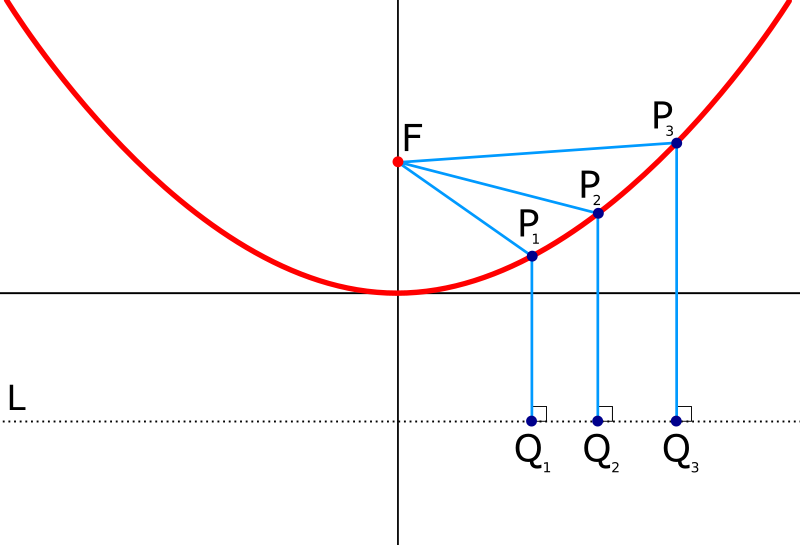
\includegraphics[scale=.3]{fig/parabola.png}
    \caption{Parabola with focus and directrix}
\end{figure}
\end{frame}


\begin{frame}[plain]
    \itmobackgroundsnakes{
        \vfill
        \Huge{The End}
        \vfill
        
\includegraphics[width=0.4\textwidth]{itmo/slogan.pdf}
    }
\end{frame}

\begin{frame}[noframenumbering]
\frametitle{Приложение}
    \large
    Модификатор \textbf{noframenumbering} можно использовать для дополнительных слайдов в конце, чтобы они не учитывались при нумерации.
\end{frame}


\end{document}
